\documentclass[11pt,a4paper]{article}
\usepackage[margin=26mm,headheight=15pt]{geometry}
\usepackage[T1]{fontenc}
\usepackage[utf8]{inputenc}
\usepackage{lmodern,microtype}
\usepackage{amsmath,amssymb,amsthm,mathtools}
\usepackage{booktabs,array,tabularx,longtable}
\usepackage{graphicx,xcolor,enumitem,fancyhdr}
\usepackage{xurl}
\usepackage[colorlinks=true,linkcolor=blue!45!black,citecolor=blue!45!black,
  urlcolor=blue!45!black]{hyperref}
\usepackage[nameinlink,noabbrev]{cleveref}
\hypersetup{pdftitle={Gaussian Bridges and Discrete Frontiers in Zero-Bias Occupancy},
  pdfauthor={Research article prepared with ChatGPT},
  pdfsubject={A proof of the geometric occupancy conjecture in ProveIt},
  pdfkeywords={Fabius function, zero bias, occupancy, conditional local limit theorem,
  Gaussian bridge, large deviations, logarithmic periodicity}}
\pagestyle{fancy}
\fancyhf{}
\fancyhead[L]{\small Zero-bias occupancy}
\fancyhead[R]{\small Gaussian bridges and discrete frontiers}
\fancyfoot[C]{\thepage}
\setlength{\emergencystretch}{2em}
\setlength{\parskip}{0.25em}
\setlist{itemsep=0.25em,topsep=0.4em}
\allowdisplaybreaks
\numberwithin{equation}{section}
\newtheorem{theorem}{Theorem}[section]
\newtheorem{proposition}[theorem]{Proposition}
\newtheorem{lemma}[theorem]{Lemma}
\newtheorem{corollary}[theorem]{Corollary}
\theoremstyle{definition}
\newtheorem{definition}[theorem]{Definition}
\newtheorem{question}[theorem]{Question}
\theoremstyle{remark}
\newtheorem{remark}[theorem]{Remark}
\newcommand{\E}{\mathbb E}
\newcommand{\PP}{\mathbb P}
\newcommand{\R}{\mathbb R}
\newcommand{\N}{\mathbb N}
\newcommand{\Z}{\mathbb Z}
\newcommand{\Var}{\operatorname{Var}}
\newcommand{\Cov}{\operatorname{Cov}}
\newcommand{\Law}{\mathcal L}
\newcommand{\TV}{d_{\mathrm{TV}}}
\newcommand{\csch}{\operatorname{csch}}
\newcommand{\diag}{\operatorname{diag}}
\newcommand{\ind}{\mathbf 1}
\newcommand{\KL}{\operatorname{D}}
\newcommand{\dd}{\,\mathrm d}
\newcommand{\simplex}{\mathcal P}
\newcommand{\repoURL}{https://github.com/VladimirReshetnikov/ProveIt}
\newcommand{\sourceURL}{https://github.com/VladimirReshetnikov/ProveIt/blob/a21208b3ff14a07a4c8318dbf916d543acbef043/Analysis/FabiusFunction/docs/semi-formalized-research-frontiers/drafts/representations/Fabius_Zero_Bias_Frontier_Report/Zero_Bias_Towers_and_Spectral_Peeling.tex}

\title{\textbf{Gaussian Bridges and Discrete Frontiers\\in Zero-Bias Occupancy}\\[0.6em]
\large A resolution of the geometric occupancy conjecture,\\
with sharp summability and centering criteria}
\author{Research article prepared with ChatGPT}
\date{5 October 2026}

\begin{document}
\maketitle
\begin{abstract}
An explicit conjecture in the Fabius--Rvachev research material of
\texttt{ProveIt} asks for a limit shape and Gaussian fluctuations of the
allocation of iterated zero-bias transformations among geometric uniform
summands. We prove that conjecture and strengthen it to convergence of the
entire fluctuation profile in $\ell^1$. The limiting covariance is exactly
one half of the multinomial covariance. The proof starts from an exact
representation by independent Poisson variables, each conditioned to be odd,
followed by conditioning the total allocation. A uniform lattice local limit
theorem makes this last conditioning rigorous.

The same argument gives a universal $\ell^2$ Gaussian bridge for every
positive summable weight profile, and identifies $\sum_j\sqrt{c_j}<\infty$
as the necessary and sufficient condition for tightness in $\ell^1$.
For power weights, centering at $mc_j$ has a sharp transition at exponent
two. For geometric weights, the last occupied scales have a different
limit: an explicit independent discrete field depending on the fractional
part of a logarithm. We obtain total-variation limits for the last occupied
index and the number of occupied indices, all moments of the latter, exact
phase averages, and asymptotic independence from the Gaussian bridge.
Finally, the normalized profile satisfies a full $\ell^1$ large deviation
principle with rate twice relative entropy. The article includes complete
proofs, reproducible exact and numerical checks, and a proposed research
program. The results are mathematical proofs in a research manuscript;
no Lean formalization or literature-wide priority is asserted.
\end{abstract}

\vspace{0.5em}
\noindent\textbf{Status and provenance.}
The resolved source statement is \texttt{conj:occupancy-shape} in
\emph{Zero-Bias Towers and Spectral Peeling in the Fabius--Rvachev System}
\cite{repo-report}. The repository was inspected at commit
\texttt{a21208b3ff14a07a4c8318dbf916d543acbef043}.
The proofs below do not assume any of that report's conjectures or its
endpoint asymptotic claims.

\newpage
{\small\tableofcontents}
\newpage

\section{The problem and the results}
\label{sec:intro}

\subsection{Why these occupancies occur}
The centered Fabius--Rvachev random series is
\[
Y_{1/2}=\sum_{j\ge0}2^{-j-1}U_j,
\qquad U_j\ \text{independent and uniform on }[-1,1].
\]
Its natural geometric extension is
\begin{equation}
Y_q=\sum_{j\ge0}c_jU_j,
\qquad c_j=(1-q)q^j,\quad 0<q<1.
\label{eq:geometric}
\end{equation}
The random-series viewpoint belongs to the classical study of the compactly
supported smooth function; see Arias de Reyna \cite{arias}. Zero bias is the
distributional transformation characterized by
\begin{equation}
\E[Wg(W)]=\Var(W)\E[g'(W^z)]
\label{eq:zero-bias}
\end{equation}
for a centered variable of positive finite variance. Goldstein and Reinert
introduced and developed this transformation \cite{goldstein-reinert}.
Symmetry is preserved, so it can be iterated on $Y_q$.

At level $m$, an exact representation of the transformed sum assigns an
integer $K_j^{(m)}$ to each summand, with $\sum_jK_j^{(m)}=m$.
Conditional on these allocations, the transformed digits are independent
and the $j$th digit has law $2\operatorname{Beta}(K_j^{(m)}+1,
K_j^{(m)}+1)-1$. The allocation law recorded in the repository is
\begin{equation}
\PP(K^{(m)}=k)=\frac1{Z_m(c)}
 \prod_{j\ge0}\frac{c_j^{2k_j}}{k_j!(2k_j+1)!!},
\qquad k_j\in\N_0,\quad \sum_jk_j=m.
\label{eq:allocation}
\end{equation}
Only finitely many $k_j$ are nonzero. We rederive the normalization and its
connection to zero bias in \cref{sec:model}.

For one transformation, the location probabilities are proportional to
$c_j^2$. The conjecture predicts that after many transformations the
\emph{fraction} of allocations at location $j$ approaches $c_j$ itself,
with Gaussian fluctuations of variance $mc_j(1-c_j)/2$. The change from
variance weights to amplitude weights is one of the structural features
explained by the proof.

\subsection{A complete answer to the stated conjecture}
For a sequence $x$, write $\|x\|_1=\sum_j|x_j|$.

\begin{theorem}[Geometric occupancy conjecture and global strengthening]
\label{thm:main-geometric}
Fix $0<q<1$, and use \cref{eq:geometric,eq:allocation}. Let $(Z_j)_{j\ge0}$
be independent standard normal variables and set
\begin{equation}
Z_* =\sum_{j\ge0}\sqrt{c_j}Z_j,
\qquad
G_j=\frac{\sqrt{c_j}Z_j-c_jZ_*}{\sqrt2}.
\label{eq:bridge}
\end{equation}
Then $G$ is an $\ell^1$-valued random variable and
\begin{equation}
\frac{K^{(m)}-mc}{\sqrt m}\ \Longrightarrow\ G
\quad\text{in }\ell^1.
\label{eq:l1-main}
\end{equation}
In particular,
\begin{equation}
\Cov(G_i,G_j)=\frac12(c_i\ind_{\{i=j\}}-c_ic_j),
\qquad \sum_jG_j=0\quad\text{almost surely}.
\label{eq:covariance}
\end{equation}
The profiles $K^{(m)}/m$ converge to $c$ in $\ell^1$, both in probability
and in mean. More precisely,
\begin{equation}
\lim_{m\to\infty}\sqrt m\,
\E\left\|\frac{K^{(m)}}m-c\right\|_1
=\frac1{\sqrt\pi}\sum_{j\ge0}\sqrt{c_j(1-c_j)}.
\label{eq:l1-error}
\end{equation}
\end{theorem}

The repository conjecture asks only for each fixed finite vector. Thus
\cref{eq:l1-main} proves both of its assertions and adds uniform control
over all scales. The expected total-variation distance between the two
probability profiles is one half of the expectation in \cref{eq:l1-error}.

\subsection{Further conclusions proved in this article}
The global theorem is part of a broader structure.
\begin{itemize}
\item \textbf{A sharp functional threshold.} For every infinite positive
profile $c$ of total mass one, exact saddle centering gives an $\ell^2$
Gaussian bridge. The square-root summability condition
$\sum_j\sqrt{c_j}<\infty$ is exactly the criterion for $\ell^1$ tightness
(\cref{thm:universal-l2,thm:l1-criterion}).
\item \textbf{A centering transition.} For $c_j=C(j+1)^{-\alpha}$,
centering at $mc_j$ is correct for $\alpha>2$, leaves a nonzero Gaussian
mean for $\alpha=2$, and misses the scale of the displacement for
$1<\alpha<2$ (\cref{thm:power}).
\item \textbf{An explicit geometric frontier.} Around index
$\log_{1/q}(2m(1-q))$, the allocation counts approach independent
discrete laws. The maximum occupied index and the occupied count have
phase-dependent lattice limits (\cref{thm:tail-tv,thm:defect-tv}).
\item \textbf{Exact occupied-count constants.} Its variance remains
bounded, with phase average $(2\log2-1)/\log(1/q)$; its mean has an explicit
periodic correction (\cref{prop:phase-averages}).
\item \textbf{A global entropy law.} The entire probability profile has a
large deviation principle in $\ell^1$ with good rate $2\KL(p\|c)$
(\cref{thm:ldp}).
\end{itemize}

\subsection{Relation to existing methods and novelty}
Conditioning independent components to represent a combinatorial law is an
established method; Arratia and Tavar\'e give a systematic treatment
\cite{arratia-tavare}. Infinite occupancy problems and their connections to
regular variation have an extensive literature \cite{gnedin-hansen-pitman}.
The law \cref{eq:allocation} has its own factorial weights and is not an
ordinary independent balls-in-boxes allocation. Its exact parity-conditioned
representation determines the factor $1/2$ in the Gaussian covariance and
the factor $2$ in the entropy rate.

The contribution claimed here is the resolution of an explicitly identified
repository conjecture, together with the extensions proved below. The
classical tools and the source allocation identity are credited. A search
of the relevant source, its README, and repository matches for the
conjecture label found no proof of that conjecture at the inspected
snapshot. This is a repository-relative assessment, not a proof of worldwide
priority. All theorem statements in this article have ordinary mathematical
proofs; numerical checks and informal independent reviews are supplementary
evidence, not formal proof certificates.

\section{The allocation law and its exact probabilistic representation}
\label{sec:model}

Unless a geometric profile is explicitly required, assume throughout that
\begin{equation}
c_j>0\quad(j\ge0),\qquad \sum_{j\ge0}c_j=1.
\label{eq:general-profile}
\end{equation}
This infinite positive setting makes every fixed finite block have a
complement of positive mass. Zero and finite-support cases are discussed in
\cref{rem:finite-support}.

\subsection{Normalization by moments}
Let $Y_c=\sum_jc_jU_j$ and $\mu_{2m}(c)=\E Y_c^{2m}$, with
$\mu_0(c)=1$. Absolute convergence gives $|Y_c|\le1$ almost surely, and
its moment generating function is
\begin{equation}
M_c(t)=\prod_{j\ge0}\frac{\sinh(tc_j)}{tc_j}.
\label{eq:mgf}
\end{equation}
The product converges locally uniformly for complex $t$: for small $z$,
$\sinh z/z=1+O(z^2)$, and $\sum c_j^2<\infty$.

\begin{proposition}[Coefficient normalization]
\label{prop:normalization}
The positive normalizing constant in \cref{eq:allocation} is finite and
equals
\begin{equation}
Z_m(c)=\frac{\mu_{2m}(c)}{(2m-1)!!\,m!}
=[z^m]\prod_{j\ge0}
 \frac{\sinh(c_j\sqrt{2z})}{c_j\sqrt{2z}}.
\label{eq:partition}
\end{equation}
Here $(-1)!!=1$. The expression involving $\sqrt{2z}$ is an entire
power series in $z$, with no choice of square-root branch involved.
\end{proposition}
\begin{proof}
The identity
\[
\frac{\sinh(c\sqrt{2z})}{c\sqrt{2z}}
=\sum_{k\ge0}\frac{2^kc^{2k}z^k}{(2k+1)!}
=\sum_{k\ge0}\frac{c^{2k}z^k}{k!(2k+1)!!}
\]
gives the sum of the weights on extracting the coefficient. On the other
hand, $M_c(\sqrt{2z})=\sum_m2^m\mu_{2m}(c)z^m/(2m)!$ and
$(2m)!=2^mm!(2m-1)!!$. Positivity of a single weight proves $Z_m(c)>0$.
Finite truncations and monotone convergence of the nonnegative coefficients
justify the infinite coefficient identity.
\end{proof}

\subsection{Connection to the zero-bias tower}
For an even moment generating function put
$\mathcal D=t^{-1}\mathrm d/\mathrm dt$, interpreting the origin by
continuity. Applying \cref{eq:zero-bias} to exponentials gives
\[
M_{W^z}(t)=\frac{\mathcal D M_W(t)}{\mathcal D M_W(0)}.
\]
By induction, the $m$th transformed law has moment generating function
\begin{equation}
\frac{\mathcal D^m M_W(t)}{\mathcal D^m M_W(0)},
\qquad
\mathcal D^m M_W(0)=\frac{\E W^{2m}}{(2m-1)!!}.
\label{eq:radial-derivative}
\end{equation}
The operator $\mathcal D$ is a derivation, so its multinomial product rule
applied to \cref{eq:mgf} yields the weights in
\cref{eq:allocation}. At an individual uniform digit, the $k$th transform
has density proportional to $(1-u^2)^k$ on $[-1,1]$: one integration by
parts verifies the next zero-bias identity, and induction starts with the
uniform density. This is the law $2\operatorname{Beta}(k+1,k+1)-1$.
All distributions have compact support, so equality of their entire moment
generating functions determines their laws. Finite truncation then gives
the countably infinite statement.

This argument identifies an allocation in an exact mixture for each
level. It does not require a particular chronological coupling of all
levels $m$ on one probability space.

\subsection{The parity-conditioned variables}
\begin{definition}
For $a>0$, let $B_a$ be the nonnegative integer-valued variable with
\begin{equation}
\PP(B_a=k)=\frac{a^{2k+1}}{(2k+1)!\sinh a},
\qquad k\in\N_0.
\label{eq:odd-poisson}
\end{equation}
Equivalently, $2B_a+1$ is a Poisson variable of parameter $a$, conditioned
to be odd. For $t>0$, construct independent $B_j(t)\sim B_{tc_j}$ and put
$S(t)=\sum_jB_j(t)$.
\end{definition}

\begin{theorem}[Exact conditioning identity]
\label{thm:conditioning}
The sum $S(t)$ is finite almost surely, $\PP(S(t)=m)>0$ for every
$m\ge0$, and
\begin{equation}
\Law(K^{(m)})
=\Law\bigl((B_j(t))_{j\ge0}\mid S(t)=m\bigr)
\quad\text{for every }t>0.
\label{eq:conditioning}
\end{equation}
\end{theorem}
\begin{proof}
Direct summation or logarithmic differentiation gives
\begin{equation}
\mu(a):=\E B_a=\frac{a\coth a-1}{2}\le\frac a2.
\label{eq:single-mean}
\end{equation}
Thus $\E S(t)\le t/2<\infty$. Also
\[
\prod_j\PP(B_j(t)=0)=\prod_j\frac{tc_j}{\sinh(tc_j)}>0,
\]
because the tail logarithms are $O(t^2c_j^2)$. Setting $B_0(t)=m$ and all
other coordinates to zero gives a positive-probability event with total
$m$. For any finite-support $k$ with total $m$, its product probability is
\[
\left(\prod_j\frac{tc_j}{\sinh(tc_j)}\right)
t^{2m}\prod_j\frac{c_j^{2k_j}}{(2k_j+1)!}.
\]
The first two factors are common to the conditioning event, and replacing
$(2k_j+1)!$ by $2^{k_j}k_j!(2k_j+1)!!$ adds the common factor $2^{-m}$.
This proves the identity.
\end{proof}

\begin{remark}[The countable construction matters]
The $B_j(t)$ are defined by their separate probability laws and then made
independent. They are \emph{not} obtained by conditioning one infinite
ordinary-Poisson vector on the event that every coordinate is odd. The latter
event has probability zero. The final event $S(t)=m$, in contrast, has
strictly positive probability by the preceding proof.
\end{remark}

\section{Saddle means and a uniform local limit theorem}
\label{sec:llt}

\subsection{Elementary estimates and the unique saddle}
Define
\begin{equation}
f(a)=1-\frac{2a}{e^{2a}-1},\qquad
D(t)=\sum_{j\ge0}f(tc_j),\qquad
M(t)=\E S(t),\qquad V(t)=\Var S(t).
\label{eq:deficit}
\end{equation}
We use $f(0)=0$ by continuity. The expansion at zero and the large-$a$
behavior are
\begin{align}
f(a)&=a-\frac{a^2}{3}+O(a^4),
&\mu(a)&=\frac{a^2}{6}+O(a^4), \label{eq:small-a}\\
f(a)&=1+O(ae^{-2a}),
&\mu(a)&=\frac{a-1}{2}+O(ae^{-2a}).\label{eq:large-a}
\end{align}

\begin{lemma}[Bounds and saddle identity]
\label{lem:saddle}
For $a>0$,
\begin{equation}
0<f(a)\le\min(a,1),\qquad
v(a):=\Var B_a
=\frac{a\coth a-a^2\csch^2a}{4}
\le\frac a4.
\label{eq:scalar-bounds}
\end{equation}
There is a unique $t_m>0$ satisfying $M(t_m)=m$ for every $m\ge1$, and
\begin{equation}
M(t)=\frac{t-D(t)}2,\quad
D(t)=o(t),\quad V(t)\sim\frac t4,\quad
t_m=2m+D(t_m)\sim2m.
\label{eq:saddle}
\end{equation}
If $\mu_j(t)=\mu(tc_j)$, then
\begin{equation}
\mu_j(t_m)-mc_j=\frac{c_jD(t_m)-f(t_mc_j)}2,
\qquad
\|\mu(t_m)-mc\|_1\le D(t_m).
\label{eq:centering-difference}
\end{equation}
\end{lemma}
\begin{proof}
The inequalities $f(a)>0$ and $f(a)<1$ follow from $e^{2a}>1+2a$.
The inequality $f(a)\le a$ is equivalent to $a\coth a\ge1$, which
follows from $\tanh a\le a$. Differentiating the probability generating
function, or using the exponential-family identity, gives
$v(a)=a\mu'(a)/2$ and the formula in \cref{eq:scalar-bounds}.
The upper bound is equivalent to
\[
\sinh a\cosh a-\sinh^2a\le a,
\]
whose left side is $(1-e^{-2a})/2\le a$. Strict positivity of $v(a)$
follows because $B_a$ is nondegenerate.

The series of means and variances converge locally uniformly by these
bounds and their small-$a$ expansions. Consequently $M$ is continuous and
strictly increasing, with $M'(t)=2V(t)/t>0$ and $M(t)\to0$ as
$t\downarrow0$. For each fixed $j$, $f(tc_j)/t\to0$, while
$f(tc_j)/t\le c_j$. Dominated convergence proves $D(t)=o(t)$ and hence
$M(t)\to\infty$. Similarly $v(tc_j)/t\to c_j/4$ and is bounded by
$c_j/4$, proving $V(t)/t\to1/4$. This proves existence, uniqueness, and
\cref{eq:saddle}. Finally $\mu(tc_j)=(tc_j-f(tc_j))/2$, so substituting
$t_m-2m=D(t_m)$ gives the exact centering difference; summing the triangle
inequality gives its norm bound.
\end{proof}

The quantities $\mu_j(t_m)$ are the means of the \emph{independent}
variables before conditioning. They need not equal $\E K_j^{(m)}$.
The term ``saddle centering'' will always refer to these explicitly defined
means, not to an asserted formula for the conditional means.

\subsection{A global Fourier bound}
The characteristic function of $B_a$ is
\begin{equation}
g_a(u)=\E e^{iuB_a}
=e^{-iu/2}\frac{\sinh(ae^{iu/2})}{\sinh a}.
\label{eq:characteristic}
\end{equation}
Although its numerator has this parity origin, $B_a$ itself has lattice
span one: every nonnegative integer has positive mass.

\begin{lemma}[One coordinate controls the Fourier integral]
\label{lem:fourier}
For $a\ge1$ and $|u|\le\pi$,
\begin{equation}
|g_a(u)|\le C_0\exp\left(-\frac{au^2}{2\pi^2}\right),
\qquad C_0=\frac2{1-e^{-2}}.
\label{eq:fourier-bound}
\end{equation}
Consequently there is an absolute constant $C_1$ such that
\begin{equation}
\sup_k\PP(B_a=k)\le \min(1,C_1a^{-1/2})
\quad(a>0).
\label{eq:atom-bound}
\end{equation}
\end{lemma}
\begin{proof}
For real $x,y$, $|\sinh(x+iy)|^2=\sinh^2x+\sin^2y\le\cosh^2x$.
On $|u|\le\pi$, $\cos(u/2)\ge0$, so
\[
|\sinh(ae^{iu/2})|\le e^{a\cos(u/2)},
\qquad \sinh a\ge\tfrac12(1-e^{-2})e^a.
\]
Also $1-\cos(u/2)\ge u^2/(2\pi^2)$. These give
\cref{eq:fourier-bound}. Fourier inversion and the Gaussian integral
give \cref{eq:atom-bound} for $a\ge1$; increasing $C_1$ covers
$0<a<1$ by the trivial bound one.
\end{proof}

\subsection{The local limit theorem}
For a fixed nonempty set $A\subseteq\N_0$, finite or infinite, set
\[
S_A(t)=\sum_{j\in A}B_j(t),\qquad
\mu_A(t)=\sum_{j\in A}\mu_j(t),\qquad C_A=\sum_{j\in A}c_j.
\]

\begin{theorem}[Uniform lattice local limit theorem]
\label{thm:llt}
For every such $A$,
\begin{equation}
\sup_{k\in\Z}\left|
\sqrt t\,\PP(S_A(t)=k)
-\sqrt{\frac2{\pi C_A}}
 \exp\left(-\frac{2(k-\mu_A(t))^2}{tC_A}\right)
\right|\longrightarrow0.
\label{eq:llt}
\end{equation}
In particular,
\begin{equation}
\PP(S(t_m)=m)\sim\sqrt{\frac2{\pi t_m}}
\sim\frac1{\sqrt{\pi m}}.
\label{eq:central-mass}
\end{equation}
\end{theorem}
\begin{proof}
First fix $j$. In \cref{eq:characteristic}, take $u=w/\sqrt t$ and
$a=tc_j$. The identity
$\log\sinh z=z-\log2+\log(1-e^{-2z})$ applies for positive real part.
The last logarithm is exponentially small uniformly on this scaled
argument. After centering, the logarithm of the characteristic function is
\[
tc_j\left(e^{iw/(2\sqrt t)}-1-\frac{iw}{2\sqrt t}\right)+o(1)
\longrightarrow-\frac{c_jw^2}{8}.
\]
Thus $(B_j(t)-\mu_j(t))/\sqrt t\Rightarrow N(0,c_j/4)$.
Independence gives the corresponding result for each finite sum. The
variance of a remaining tail divided by $t$ is at most one quarter of its
$c$-mass, by \cref{eq:scalar-bounds}; approximating $A$ by finite sets
therefore gives
\begin{equation}
\frac{S_A(t)-\mu_A(t)}{\sqrt t}\Rightarrow N(0,C_A/4).
\label{eq:sum-clt}
\end{equation}

Choose a fixed $j_0\in A$. All other characteristic factors have modulus
at most one. By \cref{lem:fourier}, after $u=w/\sqrt t$ the centered
Fourier kernel of $S_A(t)$ is bounded in modulus by
$C_0\exp(-c_{j_0}w^2/(2\pi^2))$ on $|w|\le\pi\sqrt t$.
Extend that kernel by zero outside this interval. Equation
\cref{eq:sum-clt} gives pointwise convergence to $e^{-C_Aw^2/8}$,
and dominated convergence gives convergence in $L^1(\R)$.
Fourier inversion now yields \cref{eq:llt}. Uniformity in $k$ follows
because the absolute difference of the inversions is bounded by the
$L^1$ difference of their kernels, independently of the oscillating factor.
The full set $A=\N_0$ has $C_A=1$ and mean $m$ at $t_m$, proving
\cref{eq:central-mass}.
\end{proof}

An ordinary central limit theorem alone would not justify conditioning on
$S(t_m)=m$, whose probability tends to zero. The local theorem supplies
both its precise mass and the likelihood ratios needed next.

\section{Gaussian bridges in sequence spaces}
\label{sec:bridges}

\subsection{Conditioning a fixed block}
\begin{proposition}[Finite-coordinate bridge]
\label{prop:finite-clt}
For every fixed finite $I\subset\N_0$,
\begin{equation}
\left(\frac{K_j^{(m)}-\mu_j(t_m)}{\sqrt m}\right)_{j\in I}
\Rightarrow N\left(0,\frac12\bigl(\diag(c_I)-c_Ic_I^{\mathsf T}\bigr)\right).
\label{eq:finite-clt}
\end{equation}
\end{proposition}
\begin{proof}
Let $R=\N_0\setminus I$ and $C_R=\sum_{j\in R}c_j>0$.
At $t=t_m$, the independent block's likelihood ratio under conditioning is
\[
r_t(k)=\frac{\PP(S_R(t)=m-\sum_{j\in I}k_j)}{\PP(S(t)=m)}.
\]
Set $z_j=(k_j-\mu_j(t))/\sqrt t$. Since the total mean is $m$,
the centered argument in the numerator is $-\sqrt t\sum_{j\in I}z_j$.
The uniform local theorem gives, uniformly in $k$,
\begin{equation}
r_t(k)=C_R^{-1/2}
\exp\left(-\frac{2(\sum_{j\in I}z_j)^2}{C_R}\right)+o(1).
\label{eq:ratio}
\end{equation}
These ratios are uniformly bounded. The independent block converges to a
normal vector with covariance $\diag(c_I)/4$. Hence its conditional limit
has the normal density multiplied by the bounded continuous factor in
\cref{eq:ratio}. Combining the quadratic forms, or applying the
rank-one inverse formula, gives covariance
$(\diag(c_I)-c_Ic_I^{\mathsf T})/4$ on the $\sqrt t$ scale.
Finally $t_m/m\to2$, proving \cref{eq:finite-clt}.
\end{proof}

\subsection{A bound uniform in the omitted coordinate}
\begin{lemma}[Uniform marginal domination]
\label{lem:domination}
There is a constant $C_c<\infty$ such that, for all sufficiently large
$m$, every $j\ge0$, and every nonnegative function $u$ on $\N_0$,
\begin{equation}
\E u(K_j^{(m)})\le C_c\E u(B_j(t_m)).
\label{eq:domination}
\end{equation}
In particular,
\begin{equation}
\E(K_j^{(m)}-\mu_j(t_m))^2\le C_ct_mc_j/4.
\label{eq:second-bound}
\end{equation}
\end{lemma}
\begin{proof}
If $j\ne0$, the complementary sum retains coordinate $0$; if $j=0$,
it retains coordinate $1$. A convolution's maximal atom is no larger
than that of any factor. By \cref{eq:atom-bound}, therefore,
\[
\sup_{j,k}\PP(S(t)-B_j(t)=k)\le C t^{-1/2},
\]
with a constant depending only on $c_0,c_1$. Divide this by
\cref{eq:central-mass} in the exact conditional marginal formula.
Then apply \cref{eq:scalar-bounds} to obtain \cref{eq:second-bound}.
\end{proof}

\subsection{A universal Hilbert-space limit}
The series $Z_*$ in \cref{eq:bridge} converges in $L^2$ and almost surely,
since its independent summands have total variance one. The resulting
$G$ satisfies
\begin{equation}
\E\|G\|_2^2=\frac12\left(1-\sum_jc_j^2\right)<\infty.
\label{eq:bridge-l2}
\end{equation}

\begin{theorem}[Universal $\ell^2$ bridge]
\label{thm:universal-l2}
Under \cref{eq:general-profile}, without additional tail assumptions,
\begin{equation}
\frac{K^{(m)}-\mu(t_m)}{\sqrt m}\Rightarrow G
\quad\text{in }\ell^2.
\label{eq:l2-clt}
\end{equation}
\end{theorem}
\begin{proof}
The vectors have the finite-dimensional limits in
\cref{prop:finite-clt}. By \cref{eq:second-bound},
\[
\E\sum_{j>J}\frac{|K_j^{(m)}-\mu_j(t_m)|^2}{m}
\le C\sum_{j>J}c_j\longrightarrow0
\]
uniformly for large $m$. The same tail bound holds for $G$ by its
covariance. Approximating both vectors by their first $J+1$ coordinates
proves convergence against bounded Lipschitz functions on $\ell^2$,
and hence weak convergence.
\end{proof}

\subsection{The sharp \texorpdfstring{$\ell^1$}{l1} criterion}
\begin{theorem}[Necessary and sufficient square-root summability]
\label{thm:l1-criterion}
The family $(K^{(m)}-\mu(t_m))/\sqrt m$ is tight in $\ell^1$ if and
only if
\begin{equation}
\sum_{j\ge0}\sqrt{c_j}<\infty.
\label{eq:sqrt-summable}
\end{equation}
Under this condition,
\begin{equation}
\frac{K^{(m)}-mc}{\sqrt m}\Rightarrow G
\quad\text{in }\ell^1,
\label{eq:general-l1}
\end{equation}
and \cref{eq:l1-error} holds for this general profile. If
\cref{eq:sqrt-summable} fails, the vectors centered at $mc$ are not
tight in $\ell^1$ either.
\end{theorem}
\begin{proof}
Assume first \cref{eq:sqrt-summable}. By Minkowski's inequality and
\cref{eq:second-bound},
\begin{equation}
\left\|\sum_{j>J}\frac{|K_j^{(m)}-\mu_j(t_m)|}{\sqrt m}\right\|_{L^2}
\le C\sum_{j>J}\sqrt{c_j}.
\label{eq:l1-tail}
\end{equation}
Thus finite-dimensional convergence upgrades to $\ell^1$ convergence.
The limiting $G$ belongs to $\ell^1$ because
$\E\sum_j\sqrt{c_j}|Z_j|<\infty$ and $\sum_jc_j|Z_*|=|Z_*|$.

To replace the centering, use
\[
\frac{f(tc_j)}{\sqrt t}
\le\min(\sqrt t\,c_j,t^{-1/2})\le\sqrt{c_j}.
\]
Each term tends to zero. Dominated convergence gives
$D(t)=o(\sqrt t)$, and \cref{eq:centering-difference} then gives
$\|\mu(t_m)-mc\|_1=o(\sqrt m)$. This proves
\cref{eq:general-l1}. Taking $J=-1$ in \cref{eq:l1-tail} supplies
uniform second moments of the norms, including the negligible deterministic
shift. Thus the norms are uniformly integrable and
\[
\lim_m\E\left\|\frac{K^{(m)}-mc}{\sqrt m}\right\|_1
=\E\|G\|_1
=\frac1{\sqrt\pi}\sum_j\sqrt{c_j(1-c_j)}.
\]

For necessity, suppose $\sum\sqrt{c_j}=\infty$.
The partial sums of
\[
\sum_j\sqrt{c_j}\bigl(|Z_j|-\E|Z_0|\bigr)
\]
form an $L^2$-bounded martingale and converge almost surely, since
$\sum c_j<\infty$. Therefore $\sum_j\sqrt{c_j}|Z_j|=\infty$
almost surely. Subtracting the summable vector $(c_jZ_*)_j$ cannot change
this, so $G\notin\ell^1$ almost surely. If the saddle-centered family
were tight in $\ell^1$, a subsequential limit would be an $\ell^1$-valued
random vector with the finite-dimensional laws of $G$, an impossibility.

For centering at $mc$, tightness of even coordinate zero would force
$D(t_m)/\sqrt m$ to remain bounded, by
\cref{eq:centering-difference,eq:finite-clt}. Along a subsequence it
would then converge to a finite $d\ge0$. The finite-dimensional limiting
law would be $G+(d/2)c$, since $f(t_mc_j)/\sqrt m\to0$ for fixed $j$.
Adding this summable deterministic vector still does not give an
$\ell^1$ vector. The same contradiction proves the last assertion.
\end{proof}

For geometric weights,
$\sum_j\sqrt{c_j}=\sqrt{1-q}/(1-\sqrt q)<\infty$.
The general theorem therefore proves \cref{thm:main-geometric}.

\begin{remark}[Finite support and zero weights]
\label{rem:finite-support}
Zero weights can be discarded. With exactly one positive weight,
$K_0^{(m)}=m$ is deterministic. With finitely many positive weights,
the proof first observes all but one coordinate and then recovers the
last from the total; the full covariance is singular in the expected
direction. Every summability condition is automatic. The infinite positive
assumption is used to avoid repeating these elementary cases.
\end{remark}

\section{Geometric saddles and logarithmic phase}
\label{sec:geometric-saddle}

Return to $c_j=(1-q)q^j$. Write
\[
b=1/q>1,\qquad L=\log b,\qquad x=t(1-q),\qquad
\lambda=\log_bx=n+\theta,
\]
where $n=\lfloor\lambda\rfloor$ and $0\le\theta<1$.
The sites where $tc_j$ is close to one have $j$ close to $n$.
Their exact rescaled parameters are
\begin{equation}
tc_{n+r}=q^{r-\theta}.
\label{eq:frontier-parameter}
\end{equation}
This identity explains why a fractional logarithm remains in the limit.

\begin{proposition}[An explicit smooth saddle correction]
\label{prop:saddle-phase}
Define, initially for $0\le\theta\le1$,
\begin{equation}
Q_q(\theta)=1-\theta
 +\sum_{r\le0}\bigl(f(q^{r-\theta})-1\bigr)
 +\sum_{r\ge1}f(q^{r-\theta}).
\label{eq:saddle-phase}
\end{equation}
It extends to a smooth one-periodic function. As $t\to\infty$,
\begin{equation}
D(t)=\log_b(t(1-q))+Q_q(\log_b(t(1-q)))
 +O_q\bigl(t e^{-2t(1-q)/q}\bigr).
\label{eq:deficit-phase}
\end{equation}
In particular,
\begin{align}
t_m={}&2m+\log_b(2m(1-q))
 +Q_q(\log_b(2m(1-q)))
 +O_q\left(\frac{\log m}{m}\right),
\label{eq:t-phase}\\
V(t)&=\frac t4+O_q(1).
\label{eq:geometric-variance}
\end{align}
Periodic functions are evaluated on real arguments through their periodic
extensions.
\end{proposition}
\begin{proof}
For $r\to+\infty$, the summands in \cref{eq:saddle-phase} and every
fixed-order $\theta$ derivative are $O_q(q^r)$, by
\cref{eq:small-a}. For $r\to-\infty$, the differences from one and
their derivatives decay faster than an exponential in $|r|$, by
\cref{eq:large-a}. The series and all derivatives therefore converge
uniformly. Shifting $r$ by one proves $Q_q(\theta+1)=Q_q(\theta)$,
including matching derivatives at the endpoints.

For $n\ge0$, reindex the exact deficit as
\[
D(t)=\sum_{r=-n}^{\infty}f(q^{r-\theta}).
\]
Subtract $n+1$ from the terms with $r\le0$ and compare with
\cref{eq:saddle-phase}. The omitted negative-index tail is bounded by
a constant times $(x/q)e^{-2x/q}$, since $1-f(a)=2a/(e^{2a}-1)$.
This gives \cref{eq:deficit-phase} and $D(t)=O_q(\log t)$.

The same estimates after differentiation give $D'(t)=O_q(t^{-1})$.
From $t_m-2m=D(t_m)=O_q(\log m)$, the mean-value theorem gives
$D(t_m)=D(2m)+O_q((\log m)/m)$, proving \cref{eq:t-phase}.
Finally $M'(t)=2V(t)/t$ and $M(t)=(t-D(t))/2$ imply
$V(t)=t(1-D'(t))/4$, proving \cref{eq:geometric-variance}.
\end{proof}

Geometric harmonic sums often produce logarithmic periodicity; Mellin
methods provide a broad framework \cite{flajolet-gourdon-dumas}. Here the
explicit two-sided series proves everything needed without a contour
shift, a zeta-function zero claim, or an imported endpoint expansion.

For the rest of the geometric analysis use the exact definitions
\begin{equation}
n_m=\left\lfloor\log_b(t_m(1-q))\right\rfloor,
\qquad
\theta_m=\log_b(t_m(1-q))-n_m.
\label{eq:phase-definition}
\end{equation}
Replacing this floor by an asymptotically close real expression without
tracking possible boundary crossings would be incorrect. Our moving-phase
statements keep \cref{eq:phase-definition} exactly.

\section{The discrete frontier and occupied-count laws}
\label{sec:frontier}

\subsection{The complete right-hand tail}
Let $\TV$ denote total-variation distance, normalized as one half of the
$L^1$ distance between probability mass functions. For an integer $s$ and
a real phase $\theta$, define independent variables
\begin{equation}
Z_r^{(\theta)}\sim B_{a_r(\theta)},\qquad
a_r(\theta)=q^{r-\theta},\qquad r\ge s.
\label{eq:frontier-law}
\end{equation}
The sum of these variables is finite almost surely. Indeed, their means
are $O_q(q^{2r})$ as $r\to+\infty$.

\begin{theorem}[Total-variation approximation of the moving tail]
\label{thm:tail-tv}
For every fixed integer $s$,
\begin{equation}
\TV\left(
 \Law((K_{n_m+r}^{(m)})_{r\ge s}),
 \bigotimes_{r\ge s}\Law(Z_r^{(\theta_m)})
\right)\longrightarrow0.
\label{eq:tail-tv}
\end{equation}
For sufficiently large $m$, all indices on the left are nonnegative.
Along any subsequence with $\theta_m\to\theta$, the right-hand product
may be replaced by its fixed-phase version at $\theta$.
\end{theorem}
\begin{proof}
Before conditioning, the tail beginning at $n_m+s$ has exactly the
product law on the right, by \cref{eq:frontier-parameter}. Denote its
total by $T_m$. For fixed $s$, $\E T_m$ and $\Var T_m$ are bounded
uniformly in $m$, since $0\le\theta_m<1$.

The head $S_{\mathrm h}=S-T_m$ has centered normal limit with variance
coefficient $1/4$ on the $\sqrt t$ scale. To see this, its difference from
the full centered sum is $(T_m-\E T_m)/\sqrt t\to0$ in $L^2$.
For large $m$, the head contains coordinate zero, which supplies the
Fourier bound in \cref{lem:fourier}. The proof of \cref{thm:llt}
therefore applies to this moving head as well. Its mean is
$m-\E T_m$, and its local probabilities at $m-k$, for bounded $k$,
are asymptotic to $\sqrt{2/(\pi t_m)}$ uniformly on such $k$-sets.

The conditional tail law has density
\[
R_m(T_m)=\frac{\PP(S_{\mathrm h}=m-T_m)}{\PP(S=m)}
\]
with respect to its independent product law. The local theorem gives
$R_m(k)\to1$ uniformly for bounded $k$, and the head's retained
coordinate gives a uniform upper bound on $R_m$. The totals $T_m$ are
tight, so $\E|R_m(T_m)-1|\to0$. This proves \cref{eq:tail-tv}.

To vary the phase, truncate at a large right endpoint $R$. On a finite
coordinate set the product probabilities depend continuously, in total
variation, on $\theta$. The probability of any nonzero coordinate beyond
$R$ is $O_q(q^{2R})$ uniformly for $\theta\in[0,1]$, so the complete products are
also continuous in total variation.
\end{proof}

\subsection{A two-sided occupancy interface}
For $r\in\Z$ define
\begin{equation}
b_r(\theta)=\PP(Z_r^{(\theta)}=0)
=\frac{a_r(\theta)}{\sinh a_r(\theta)}.
\label{eq:vacancy}
\end{equation}
We may construct all $Z_r^{(\theta)}$, $r\in\Z$, independently.
Their actual count sequence is not summable to the left. Their
\emph{deviations from an occupied-left, vacant-right pattern}, however,
are finite:
\begin{equation}
\mathcal D_\theta(r)
=\ind_{\{Z_r^{(\theta)}>0\}}-\ind_{\{r\le0\}}.
\label{eq:limit-defect}
\end{equation}
Indeed,
\begin{equation}
\sum_{r\le0}b_r(\theta)+\sum_{r\ge1}(1-b_r(\theta))<\infty,
\label{eq:defect-sum}
\end{equation}
uniformly for $\theta\in[0,1]$. The left tail decreases faster than
exponentially in $|r|$, and the right tail is $O_q(q^{2r})$.
The first Borel--Cantelli lemma implies finite support almost surely.

For the conditioned model, take $m$ sufficiently large that $n_m\ge0$ and set
\begin{equation}
\mathcal D_m(r)=
\begin{cases}
\ind_{\{K_{n_m+r}^{(m)}>0\}}-\ind_{\{r\le0\}},&r\ge-n_m,\\
0,&r<-n_m.
\end{cases}
\label{eq:finite-defect}
\end{equation}
The extension by zero records no artificial vacancies before the original
index zero.

\begin{lemma}[Uniform bounds for any number of omitted sites]
\label{lem:multi-domination}
There exists $C_q<\infty$ such that, for all sufficiently large $m$,
every finite set $A\subset\N_0$ with $|A|=p$, and coordinate events
$E_j\subseteq\N_0$,
\begin{equation}
\PP(K_j^{(m)}\in E_j\text{ for all }j\in A)
\le C_q q^{-p/2}\prod_{j\in A}\PP(B_j(t_m)\in E_j).
\label{eq:multi-domination}
\end{equation}
\end{lemma}
\begin{proof}
The complement of $A$ contains some $\ell\in\{0,\ldots,p\}$.
Its sum has maximal atom at most
$C_1(t_m(1-q)q^p)^{-1/2}$ by \cref{eq:atom-bound}.
Condition on the coordinates in $A$, use their independence, and divide
by \cref{eq:central-mass}. This gives the stated constant independently
of $A,p$, including when the displayed upper bound exceeds one.
\end{proof}

\begin{theorem}[The full defect field and its functionals]
\label{thm:defect-tv}
On the countable space of finitely supported $\{-1,0,1\}$-valued
sequences on $\Z$,
\begin{equation}
\TV(\Law(\mathcal D_m),\Law(\mathcal D_{\theta_m}))\longrightarrow0.
\label{eq:defect-tv}
\end{equation}
Let
\[
M_m=\max\{j:K_j^{(m)}>0\},\qquad
H_m=\#\{j:K_j^{(m)}>0\},
\]
and define
\begin{equation}
W_\theta=\sup\{r:Z_r^{(\theta)}>0\},\qquad
L_\theta=-\sum_{r\le0}\ind_{\{Z_r^{(\theta)}=0\}}
 +\sum_{r\ge1}\ind_{\{Z_r^{(\theta)}>0\}}.
\label{eq:frontier-functionals}
\end{equation}
Then the law of $(M_m-n_m,H_m-(n_m+1))$ is asymptotic in total variation
to the law of $(W_{\theta_m},L_{\theta_m})$. For $s\in\Z$,
\begin{equation}
\PP(W_\theta\le s)=\prod_{r>s}b_r(\theta),
\label{eq:max-cdf}
\end{equation}
and, for real $u$,
\begin{equation}
\E e^{uL_\theta}
=\prod_{r\le0}(1-b_r+b_re^{-u})
 \prod_{r\ge1}(b_r+(1-b_r)e^u).
\label{eq:count-mgf}
\end{equation}
All moments and all real exponential moments of $H_m-(n_m+1)$ converge
to the corresponding moving-phase expressions in \cref{eq:count-mgf}.
\end{theorem}
\begin{proof}
The case $p=1$ of \cref{lem:multi-domination} and a union bound show
that the probability of any defect outside $[-R,R]$ is at most a constant
times
\[
\sum_{r<-R}b_r(\theta_m)+\sum_{r>R}(1-b_r(\theta_m)),
\]
which tends uniformly to zero as $R\to\infty$. The same bound holds
for the independent limiting field by \cref{eq:defect-sum}.
On $[-R,R]$, \cref{thm:tail-tv} gives total-variation convergence.
Extend these truncated fields by zero and then let $R\to\infty$;
the triangle inequality proves \cref{eq:defect-tv}.

For these sufficiently large $m$, the sum of the field is $H_m-(n_m+1)$. Its occupied pattern, interpreted
as the baseline $\ind_{\{r\le0\}}$ plus the field, has maximum
$M_m-n_m$ for $m\ge1$; artificial occupied sites to the far left do not
alter that maximum. Thus the joint functional assertion follows by
contraction of total variation. Independence of the $Z_r$ proves
\cref{eq:max-cdf,eq:count-mgf}; their products converge by
\cref{eq:defect-sum}. The maximum is finite almost surely, and the
pattern has occupied sites arbitrarily far to the left.

It remains to justify the unbounded moment statements. Let
$N_m=\sum_r|\mathcal D_m(r)|$, and let $d_{j,m}$ be the corresponding
unconditioned defect probability at original site $j$. Equation
\cref{eq:defect-sum} gives $\sum_jd_{j,m}\le A_q$ for a finite
constant $A_q$ independent of $m$. Summing
\cref{eq:multi-domination} over sets of $p$ defect sites yields
\[
\E\binom{N_m}{p}
\le C_q q^{-p/2}\frac{A_q^p}{p!}.
\]
For $v\ge0$, expand $(1+(e^v-1))^{N_m}$ to obtain
\begin{equation}
\E e^{vN_m}\le C_q
 \exp\bigl(q^{-1/2}A_q(e^v-1)\bigr).
\label{eq:defect-exp}
\end{equation}
The independent fields obey an analogous uniform bound. Since
$|H_m-(n_m+1)|\le N_m$, these estimates imply uniform integrability
of every power and every fixed real exponential, using a larger
exponent in \cref{eq:defect-exp}. Total-variation convergence followed
by truncation proves the moment assertions.
\end{proof}

\begin{corollary}[A sharp far-right tail]
\label{cor:max-tail}
For fixed phase, as the integer $s\to+\infty$,
\begin{equation}
\PP(W_\theta>s)
\sim\frac{q^{2(s+1-\theta)}}{6(1-q^2)}.
\label{eq:max-tail}
\end{equation}
The maximum's limit law depends nontrivially on phase.
\end{corollary}
\begin{proof}
As $a\downarrow0$, $a/\sinh a=1-a^2/6+O(a^4)$.
Taking logarithms in \cref{eq:max-cdf} gives the geometric sum in
\cref{eq:max-tail}, with error $O_q(q^{4s})$. Phase dependence is
strict: increasing $\theta$ increases every $a_r$, and $a/\sinh a$
strictly decreases for $a>0$, so the CDF in \cref{eq:max-cdf} strictly
decreases at every fixed integer $s$.
\end{proof}

\subsection{Mean, variance, and exact phase averages}
Define
\begin{equation}
h_q(\theta)=-\sum_{r\le0}b_r(\theta)
 +\sum_{r\ge1}(1-b_r(\theta)),\qquad
v_q(\theta)=\sum_{r\in\Z}b_r(\theta)(1-b_r(\theta)).
\label{eq:count-functions}
\end{equation}
These are smooth; $h_q(\theta+1)=h_q(\theta)+1$ and
$v_q(\theta+1)=v_q(\theta)$. The moment convergence just proved gives
\begin{equation}
\E H_m=n_m+1+h_q(\theta_m)+o(1),\qquad
\Var H_m=v_q(\theta_m)+o(1).
\label{eq:count-moments}
\end{equation}

\begin{proposition}[Exact averages and mean expansion]
\label{prop:phase-averages}
One has
\begin{equation}
\int_0^1h_q(\theta)\dd\theta=-\frac{\log2}{L},\qquad
\int_0^1v_q(\theta)\dd\theta=\frac{2\log2-1}{L}.
\label{eq:phase-averages}
\end{equation}
The function
\begin{equation}
P_q(\theta)=h_q(\theta)-\theta+\frac12+\frac{\log2}{L}
\label{eq:count-periodic}
\end{equation}
is smooth, one-periodic, and mean zero. Moreover,
\begin{equation}
\E H_m=\log_b((1-q)m)+\frac12
 +P_q\bigl(\log_b(2(1-q)m)\bigr)+o(1).
\label{eq:mean-count}
\end{equation}
For $q=1/2$ this specializes to
\begin{equation}
\E H_m=\log_2m-\frac12+P_{1/2}(\log_2m)+o(1),\qquad
\int_0^1v_{1/2}(\theta)\dd\theta=2-\frac1{\log2}.
\label{eq:dyadic-count}
\end{equation}
\end{proposition}
\begin{proof}
Uniformly convergent tail bounds justify integration term by term.
The change of variable $a=q^{r-\theta}$ tiles $(0,\infty)$ as $r$
varies and $\theta$ runs from zero to one. Thus
\[
L\int_0^1h_q(\theta)\dd\theta
=\int_0^1\left(\frac1a-\frac1{\sinh a}\right)\dd a
 -\int_1^\infty\frac{\dd a}{\sinh a}=-\log2,
\]
using $\int\csch a\dd a=\log\tanh(a/2)$ and the limit
$\tanh(a/2)\sim a/2$ at zero. Similarly,
\[
L\int_0^1v_q(\theta)\dd\theta
=\int_0^\infty\left(\csch a-a\csch^2a\right)\dd a
=2\log2-1.
\]
An antiderivative for the latter integrand is
$\log\tanh(a/2)+a\coth a-\log\sinh a$; its limits at infinity
and zero are $\log2$ and $1-\log2$.

The shift identity for $h_q$ follows by reindexing the series, and
\cref{eq:phase-averages} then proves the assertions about $P_q$.
Substituting \cref{eq:count-periodic} in \cref{eq:count-moments}
gives
\[
\E H_m=\log_b(t_m(1-q))+\tfrac12-\log_b2
 +P_q(\log_b(t_m(1-q)))+o(1).
\]
Since $t_m/(2m)=1+O_q((\log m)/m)$ and $P_q$ has bounded derivative,
this is \cref{eq:mean-count}.
\end{proof}

The variance function is bounded above and bounded away from zero: its
series is continuous on the phase circle, and each value contains positive
terms. Thus the fluctuations of $H_m-\log_bm$ have order one. They do
not have a nondegenerate Gaussian limit after division by
$\sqrt{\log m}$. This distinction separates the frontier from the
macroscopic Gaussian fluctuations of $K_j^{(m)}$.

\subsection{Independence of the two limiting scales}
\begin{theorem}[The bridge and the frontier become independent]
\label{thm:independence}
Along every subsequence with $\theta_m\to\theta$,
\begin{equation}
\left(\frac{K^{(m)}-mc}{\sqrt m},\mathcal D_m\right)
\Rightarrow (G,\mathcal D_\theta)
\label{eq:joint-limit}
\end{equation}
in the product of $\ell^1$ and the discrete space of finite defect fields.
The two random elements on the right are independent.
\end{theorem}
\begin{proof}
Fix a macroscopic block $I=\{0,\ldots,J\}$ and a frontier tail
beginning at $n_m+s$. For large $m$ they are disjoint. Before conditioning,
the block, the tail, and the intervening remaining coordinates are
independent. The tail's total is uniformly tight. The remaining sum has a
local limit theorem with variance coefficient
$(1-\sum_{i\in I}c_i)/4$: deleting the tail changes the fixed complement
by a variable of bounded variance, and an unused fixed coordinate such as
$J+1$ supplies the Gaussian Fourier bound.

If $z_i=(k_i-\mu_i(t_m))/\sqrt{t_m}$ and the tail has bounded total,
the conditional likelihood ratio therefore tends, uniformly for $z$ in
compact sets, to
\[
\left(1-\sum_{i\in I}c_i\right)^{-1/2}
\exp\left[-\frac{2(\sum_{i\in I}z_i)^2}
 {1-\sum_{i\in I}c_i}\right].
\]
This limit does not depend on the tail. The ratios are uniformly bounded
by the same retained-coordinate estimate. Truncating the tight tail total
and then the tight block coordinates proves the product of the finite
Gaussian bridge law and the independent tail law.

The defect bounds outside $[-R,R]$ used in
\cref{thm:defect-tv} extend this product convergence to the whole
defect field. Finally \cref{eq:l1-tail} extends the finite Gaussian
block to $\ell^1$. The deterministic centering difference is
$O_q(\log m)/\sqrt m$ in $\ell^1$, so the centering by $mc$ in
\cref{eq:joint-limit} is valid.
\end{proof}

\section{The sharp centering transition for power weights}
\label{sec:power}

The geometric theorem might suggest that centering by $mc_j$ works for
every summable profile. The exact saddle identity shows that this is false.
It also identifies the relevant threshold without changing the random
fluctuation mechanism.

\begin{proposition}[General centering criterion]
\label{prop:centering-criterion}
For any fixed nonempty finite set of positive coordinates, the centered
Gaussian limit in \cref{eq:finite-clt} remains valid when
$\mu_j(t_m)$ is replaced by $mc_j$ if and only if
\begin{equation}
D(t_m)=o(\sqrt m).
\label{eq:centering-criterion}
\end{equation}
If $D(t_m)/\sqrt m\to d<\infty$, the limiting mean is
$(d/2)c_j$. If $D(t_m)/\sqrt m\to\infty$, each fixed coordinate
$(K_j^{(m)}-mc_j)/\sqrt m$ tends to $+\infty$ in probability.
\end{proposition}
\begin{proof}
For fixed $j$, $f(t_mc_j)\to1$. The exact difference
\cref{eq:centering-difference} is therefore a deterministic shift
of size $c_jD(t_m)/(2\sqrt m)+o(1)$ on the fluctuation scale.
The saddle-centered sequence converges to a nondegenerate centered
normal in that coordinate. The finite-shift and divergent-shift statements
follow immediately. Conversely, if \cref{eq:centering-criterion} fails,
there is a subsequence along which this nonnegative shift is bounded away
from zero and has a finite positive or infinite subsequential limit. It
cannot have the same centered normal limit.
\end{proof}

\begin{theorem}[Power-law threshold at exponent two]
\label{thm:power}
Let
\[
c_j=C(j+1)^{-\alpha},\qquad \alpha>1,\qquad C=\zeta(\alpha)^{-1}.
\]
Define the positive finite constant
\begin{equation}
A_\alpha=C^{1/\alpha}\int_0^\infty
 f(x^{-\alpha})\dd x.
\label{eq:power-constant}
\end{equation}
Then
\begin{equation}
D(t)=A_\alpha t^{1/\alpha}+O(1).
\label{eq:power-deficit}
\end{equation}
For each fixed finite block, the variables centered at $mc$ have the
following behavior:
\begin{center}
\begin{tabular}{@{}ll@{}}
\toprule
Exponent & Limit on the $\sqrt m$ scale \\
\midrule
$\alpha>2$ & Centered Gaussian bridge \\
$\alpha=2$ & Gaussian bridge with mean $c_jA_2/\sqrt2$ \\
$1<\alpha<2$ & Every fixed positive coordinate tends to $+\infty$ \\
\bottomrule
\end{tabular}
\end{center}
The $\ell^1$ bridge occurs exactly for $\alpha>2$. The universal
$\ell^2$ theorem with saddle centering holds for all $\alpha>1$.
\end{theorem}
\begin{proof}
The function $g(x)=f(x^{-\alpha})$ is decreasing from one to zero,
positive, and integrable: it is bounded near zero, and
$g(x)=O(x^{-\alpha})$ at infinity. Monotonicity follows either by
direct differentiation or from
\[
f'(a)=\frac{2((2a-1)e^{2a}+1)}{(e^{2a}-1)^2}>0.
\]
Set $s=(Ct)^{1/\alpha}$. Then
$D(t)=\sum_{n\ge1}g(n/s)$.
Comparison of a right Riemann sum with its integral gives
\[
0\le s\int_0^\infty g(x)\dd x-\sum_{n\ge1}g(n/s)\le1.
\]
This proves \cref{eq:power-deficit}, including its bounded error.
Since $t_m\sim2m$, the three regimes follow from
\cref{prop:centering-criterion}. Finally
$\sum_j\sqrt{c_j}<\infty$ holds exactly when $\alpha>2$;
apply \cref{thm:l1-criterion}.
\end{proof}

\begin{proposition}[Optional evaluation of the power-law constant]
\label{prop:power-zeta}
With $\beta=1/\alpha\in(0,1)$,
\begin{equation}
A_\alpha=-\beta(2C)^\beta\Gamma(1-\beta)\zeta(1-\beta)>0.
\label{eq:power-zeta}
\end{equation}
In particular,
\begin{equation}
A_2=-\sqrt{\frac{\pi C}{2}}\,\zeta(1/2).
\label{eq:a2}
\end{equation}
\end{proposition}
\begin{proof}
Put $F(y)=(e^y-1)^{-1}-y^{-1}$. For $0<s<1$, the integral
$I(s)=\int_0^\infty F(y)y^{s-1}\dd y$ is absolutely convergent.
The identity $F(y)-2F(2y)=(e^y+1)^{-1}$ gives
\[
(1-2^{1-s})I(s)=\int_0^\infty\frac{y^{s-1}}{e^y+1}\dd y
=\Gamma(s)\eta(s),
\]
where $\eta(s)=\sum_{n\ge1}(-1)^{n-1}n^{-s}$.
For completeness, expansion of $(e^y+1)^{-1}$ into alternating
exponentials is justified in the integral by its alternating remainder:
the integral of the remainder is at most
$\Gamma(s)(N+1)^{-s}$. The standard identity
$\eta(s)=(1-2^{1-s})\zeta(s)$, or equivalently this definition of
the continued zeta function on $(0,1)$, gives $I(s)=\Gamma(s)\zeta(s)$.
Substitute $u=x^{-\alpha}$ in \cref{eq:power-constant}, then put
$y=2u$ and use $f(u)=-2uF(2u)$. This gives
$A_\alpha=-\beta(2C)^\beta I(1-\beta)$, proving the formula.
Positivity already follows from \cref{eq:power-constant}.
\end{proof}

The positive integral in \cref{eq:power-constant} is sufficient for the
threshold theorem. The special-function evaluation adds an exact constant,
not an additional assumption.

\section{A full large deviation principle in \texorpdfstring{$\ell^1$}{l1}}
\label{sec:ldp}

The local and Gaussian theorems describe typical fluctuations. A different
exact identity determines the exponential cost of an atypical profile.
This section applies to every profile in \cref{eq:general-profile}.
Let
\[
\simplex=\{p\in\ell^1:p_j\ge0,\ \sum_jp_j=1\},\qquad P_m=K^{(m)}/m.
\]
All logarithms in relative entropy are natural logarithms. Define
\begin{equation}
\KL(p\|c)=\sum_jp_j\log\frac{p_j}{c_j}
=\sum_jc_j\phi(p_j/c_j),\qquad
\phi(x)=x\log x-x+1,
\label{eq:entropy}
\end{equation}
with $0\log0=0$ and value $+\infty$ allowed. The nonnegative second
series gives an unambiguous definition even when the entropy is infinite.

\begin{theorem}[Twice-relative-entropy large deviations]
\label{thm:ldp}
The laws of $P_m$ satisfy the full large deviation principle on
$\simplex$ with its $\ell^1$ topology, at speed $m$, with good rate
\begin{equation}
I(p)=2\KL(p\|c).
\label{eq:rate}
\end{equation}
Explicitly, for every relatively open $G\subseteq\simplex$ and relatively
closed $F\subseteq\simplex$,
\begin{align}
\liminf_{m\to\infty}\frac1m\log\PP(P_m\in G)
&\ge-\inf_{p\in G}I(p),\label{eq:ldp-lower}\\
\limsup_{m\to\infty}\frac1m\log\PP(P_m\in F)
&\le-\inf_{p\in F}I(p).
\label{eq:ldp-upper}
\end{align}
The sublevel sets of $I$ are compact in $\ell^1$.
\end{theorem}

We give the proof in several steps, including exponential tightness, so
that no change between a coordinate topology and $\ell^1$ is implicit.

\subsection{An exact exponential-tilt identity}
For any nonnegative summable profile $a$, not necessarily of total mass
one, put $\mu_{2m}(a)=\E(\sum_ja_jU_j)^{2m}$.
By independence and symmetry of finite sums and then monotone convergence
of their nonnegative coefficient expansions,
\begin{equation}
\mu_{2m}(a)=(2m)!
\sum_{\sum_jk_j=m}\prod_j\frac{a_j^{2k_j}}{(2k_j+1)!}.
\label{eq:moment-coefficients}
\end{equation}
Convergence of the random sums is uniform almost surely, so their moments
converge to the same expression.

If $\vartheta=(\vartheta_j)$ is any real sequence with
$A(\vartheta)=\sum_jc_je^{\vartheta_j/2}<\infty$, then Tonelli's
theorem applied to \cref{eq:moment-coefficients} proves
\begin{equation}
\E e^{\sum_j\vartheta_jK_j^{(m)}}
=\frac{\mu_{2m}((c_je^{\vartheta_j/2})_j)}{\mu_{2m}(c)}.
\label{eq:tilt-identity}
\end{equation}
This holds for unbounded tilts as well as bounded ones; the summability of
the tilted profile is the needed hypothesis.

For a positive total mass $A=\sum_ja_j$, compact support gives
$|\sum a_jU_j|\le A$. Conversely, for every $\varepsilon>0$ there is
positive probability that this sum exceeds $A-\varepsilon$: choose a
finite head with tail mass less than $\varepsilon/4$ and require each of
its finitely many uniform digits to be sufficiently close to one.
It follows that
\begin{equation}
\mu_{2m}(a)^{1/(2m)}\longrightarrow A.
\label{eq:endpoint-moment}
\end{equation}
Thus \cref{eq:tilt-identity} gives
\begin{equation}
\Lambda(\vartheta):=
\lim_{m\to\infty}\frac1m\log\E e^{m\langle\vartheta,P_m\rangle}
=2\log\sum_jc_je^{\vartheta_j/2}.
\label{eq:limiting-mgf}
\end{equation}
No estimate on how quickly the density vanishes at its endpoint enters
this argument.

\subsection{Finite partitions and entropy duality}
For $J\ge0$, collapse all coordinates above $J$ into a single tail cell:
\[
p^{[J]}=(p_0,\ldots,p_J,p_{>J}),\qquad
c^{[J]}=(c_0,\ldots,c_J,c_{>J}).
\]
The log-moment formula for this finite simplex is
\[
\Lambda_J(\vartheta)=2\log\left(
 \sum_{j=0}^Jc_je^{\vartheta_j/2}
 +c_{>J}e^{\vartheta_*/2}\right).
\]
Its convex dual is $I_J(p^{[J]})=2\KL(p^{[J]}\|c^{[J]})$.
For positive coordinates the optimizing tilt is
$\vartheta_i=2\log(p_i/c_i^{[J]})$, up to adding a common constant.
Zero coordinates follow by limits.

The finite-simplex large deviation bounds can be proved directly. For an
interior target $p$, tilt by the preceding $\vartheta$. The new limiting
logarithmic moment generating function is
$\Lambda_J(\vartheta+u)-\Lambda_J(\vartheta)$, with gradient $p$ at
zero. Chernoff bounds for each coordinate, using differentiability at
zero, show that the tilted law concentrates exponentially in every
neighborhood of $p$. Changing back to the original law gives lower
exponent $-\langle\vartheta,p\rangle+\Lambda_J(\vartheta)=-I_J(p)$.
For boundary targets, approach by
$(1-\varepsilon)p+\varepsilon c^{[J]}$; finite-simplex entropy is
continuous. Chernoff bounds followed by a finite cover of the compact
simplex give the upper bound. This proves both finite-dimensional bounds
without presuming nonsingularity in the direction of the total mass.

Jensen's inequality applied to $\phi$ in \cref{eq:entropy} gives
\begin{equation}
I_J(p^{[J]})\uparrow I(p).
\label{eq:entropy-partitions}
\end{equation}
Indeed each finite partition entropy is at most the full entropy, whereas
its nonnegative sum over the first $J+1$ cells already increases to the
full sum. Consequently
\begin{equation}
I(p)=\sup_{\vartheta\in\ell^\infty}
 \{\langle\vartheta,p\rangle-\Lambda(\vartheta)\}.
\label{eq:entropy-duality}
\end{equation}
For the upper inequality, apply nonnegativity of entropy to the tilted
probability profile $c_je^{\vartheta_j/2}/A(\vartheta)$; for the reverse
inequality optimize over tilts constant on each finite partition and use
\cref{eq:entropy-partitions}. Formula \cref{eq:entropy-duality}
also proves lower semicontinuity in $\ell^1$.

\subsection{Explicit exponential tightness}
Let $T_j=\sum_{k\ge j}c_k$ and
\begin{equation}
w_j=-\tfrac12\log T_j.
\label{eq:coercive-weights}
\end{equation}
Then $w_j\uparrow\infty$, $w_0=0$, and
\begin{equation}
A:=\sum_jc_je^{w_j}=\sum_j\frac{c_j}{\sqrt{T_j}}\le2.
\label{eq:coercive-bound}
\end{equation}
To verify the bound, use $c_j=T_j-T_{j+1}$ and
\[
\frac{c_j}{\sqrt{T_j}}
=(\sqrt{T_j}-\sqrt{T_{j+1}})
 \left(1+\sqrt{T_{j+1}/T_j}\right)
\le2(\sqrt{T_j}-\sqrt{T_{j+1}})
\]
and telescope. The unbounded tilt $\vartheta_j=2w_j$ is therefore
admissible in \cref{eq:limiting-mgf}. Markov's inequality yields
\begin{equation}
\limsup_m\frac1m\log\PP\left(\sum_jw_jP_{m,j}>R\right)
\le-2R+2\log A\le-2R+2\log2.
\label{eq:exp-tightness}
\end{equation}
The sets
\[
\mathcal K_R=\{p\in\simplex:\sum_jw_jp_j\le R\}
\]
are compact in $\ell^1$: they are closed, and their tails are uniformly
bounded by $R/w_{J+1}\to0$, so a coordinatewise diagonal subsequence
converges in $\ell^1$. This proves exponential tightness in the required
topology.

\subsection{Completion of the infinite-dimensional bounds}
Fix $p$ in an $\ell^1$-open set $G$. Choose a ball of radius
$\varepsilon$ about $p$ inside $G$, and take $J$ with
$2p_{>J}<\varepsilon/2$. If another probability profile $q$ satisfies
$\sum_{j\le J}|q_j-p_j|<\delta$, then
\[
\|q-p\|_1\le2\delta+2p_{>J}.
\]
For small $\delta$, this finite-coordinate cylinder lies inside $G$.
The finite-partition lower bound gives exponent at least
$-I_J(p^{[J]})\ge-I(p)$. Optimizing over $p\in G$ proves
\cref{eq:ldp-lower}.

For a compact set $C\subset\simplex$ and a real
$a<\inf_{p\in C}I(p)$, \cref{eq:entropy-duality} supplies for each
$p\in C$ a bounded tilt with
$\langle\vartheta,p\rangle-\Lambda(\vartheta)>a$.
This strict inequality holds on a neighborhood of $p$. A Chernoff bound
gives upper exponent at most $-a$ there. A finite subcover gives the
compact upper bound. For a closed $F$, apply it to $F\cap\mathcal K_R$
and use \cref{eq:exp-tightness} on the complement; letting $R\to\infty$
proves \cref{eq:ldp-upper}.

Finally, use \cref{eq:entropy-duality} with bounded truncations of
$2w_j$ to obtain
\[
I(p)\ge2\sum_jw_jp_j-2\log A.
\]
Every rate sublevel set is therefore contained in a compact $\mathcal K_R$.
Lower semicontinuity proves that it is compact. This completes the proof
of \cref{thm:ldp}.

\begin{corollary}[Exponential concentration and a strong law]
\label{cor:concentration}
For every $\varepsilon>0$,
\begin{equation}
\limsup_m\frac1m\log\PP(\|K^{(m)}/m-c\|_1\ge\varepsilon)
\le-\varepsilon^2.
\label{eq:concentration}
\end{equation}
Consequently $K^{(m)}/m\to c$ in $\ell^1$ almost surely under any
common coupling of the occupancy vectors. Independence between levels
is not required.
\end{corollary}
\begin{proof}
The case $p=c$ is immediate. Otherwise, the entropy inequality
$2\KL(p\|c)\ge\|p-c\|_1^2$ follows by collapsing to
$A=\{j:p_j>c_j\}$ and its complement, where $0<c(A)<1$. For a fixed reference probability, binary relative entropy has second
derivative $1/(x(1-x))\ge4$, so its value is at least twice the square
of the difference of the binary probabilities. That difference is
$\|p-c\|_1/2$. Apply the large deviation upper bound to the closed set
in \cref{eq:concentration}. For each fixed $\varepsilon>0$ the
probabilities are summable, and Borel--Cantelli, followed by countably
many $\varepsilon$, proves the strong law.
\end{proof}

The quadratic expansion of $2\KL(p\|c)$ about $c$ is consistent with
the half-multinomial Gaussian covariance. The Gaussian theorem was proved
separately: differentiating a limiting logarithmic moment generating
function alone would not have justified it.

\section{Reproducible exact and numerical checks}
\label{sec:numerics}

The companion program \texttt{verify\_occupancy.py} uses exact rational
arithmetic for small levels and positive recurrences in logarithmic
arithmetic for larger levels. It uses no Monte Carlo. All tables and
figures in this section are reproducible from the included source and
CSV files. The numerical calculations test finite identities and illustrate
limits; the preceding proofs establish the asymptotic statements.

\subsection{A positive moment recurrence and an exact marginal}
For geometric weights, $Y_q\overset d=(1-q)U+qY_q'$, independently.
Write $\mu_r=\E Y_q^{2r}$. Expanding the even moment and isolating the
self-term gives
\begin{equation}
(1-q^{2m})\mu_m
=\sum_{k=1}^m\binom{2m}{2k}
 \frac{(1-q)^{2k}q^{2(m-k)}}{2k+1}\mu_{m-k},\qquad \mu_0=1.
\label{eq:moment-recurrence}
\end{equation}
Here and only in this computational subsection the subscript $m$ on
$\mu_m$ denotes the $2m$th moment. Coefficient extraction gives
\begin{equation}
\PP_m(K_0=k)=\binom{2m}{2k}
 \frac{(1-q)^{2k}q^{2(m-k)}\mu_{m-k}}{(2k+1)\mu_m},
\qquad 0\le k\le m.
\label{eq:exact-marginal}
\end{equation}
In particular $\PP_m(K_0=0)=q^{2m}$ exactly.
Conditional on $K_0=k$, the remaining coordinates, reindexed from zero,
have the same occupancy law with total $m-k$. This follows because
multiplying every tail weight by the same $q$ contributes a common
factor for the fixed residual total.

This self-similarity computes the covariance of $K_0,K_1$ without
truncating the infinite digit set. It also yields an exact residual-total
chain for computing the expected $\ell^1$ error and a recursion for the
occupied count. For the latter, empty first sites can be skipped: conditional
on $K_0>0$, the occupied count is $1+H_{m-K_0}$, and the empty-site
case has the original $H_m$ law. Solving for the mean and variance gives
the recurrences used by the program.

The exact checks use \texttt{fractions.Fraction} at $q=1/2$ through
$m=12$. They verify positivity, normalization, the vacancy identity,
direct two-head coefficient extraction, the conditional self-similarity,
the covariance formula, and monotonicity of exact maximum-index CDFs.

\begin{table}[htbp]
\centering
\caption{Dyadic allocations computed from the positive moment recurrence.
The final row gives the limits from the bridge theorem.}
\label{tab:bulk}
\small
\begin{tabular}{@{}rrrr@{}}
\toprule
$m$ & $\E K_0/m$ & $\Var(K_0)/m$ & $\Cov(K_0,K_1)/m$ \\
\midrule
16 & 0.5587271132 & 0.1416368701 & $-0.0766758432$ \\
64 & 0.5218299035 & 0.1309863936 & $-0.0669174041$ \\
256 & 0.5073515386 & 0.1269729311 & $-0.0638397003$ \\
1024 & 0.5023213920 & 0.1256142933 & $-0.0628952716$ \\
\midrule
Limit & $1/2$ & $1/8$ & $-1/16$ \\
\bottomrule
\end{tabular}
\end{table}

\begin{remark}[Why moment comparisons have the stated limits]
The finite-coordinate CLT also permits second-moment convergence here.
For fixed $j$, logarithmic differentiation of
\cref{eq:characteristic}, using the large-$a$ expansion, gives
$\E(B_a-\mu(a))^4=O(a^2)$ as $a\to\infty$.
The marginal domination bound transfers this to
$\E(K_j-\mu_j(t_m))^4=O(m^2)$.
Thus the squared normalized coordinates and their products are uniformly
integrable. Their limiting variances and covariances are indeed those in
\cref{eq:covariance}, not merely suggestive quantities extracted from a
weak limit.
\end{remark}

\begin{figure}[htbp]
\centering
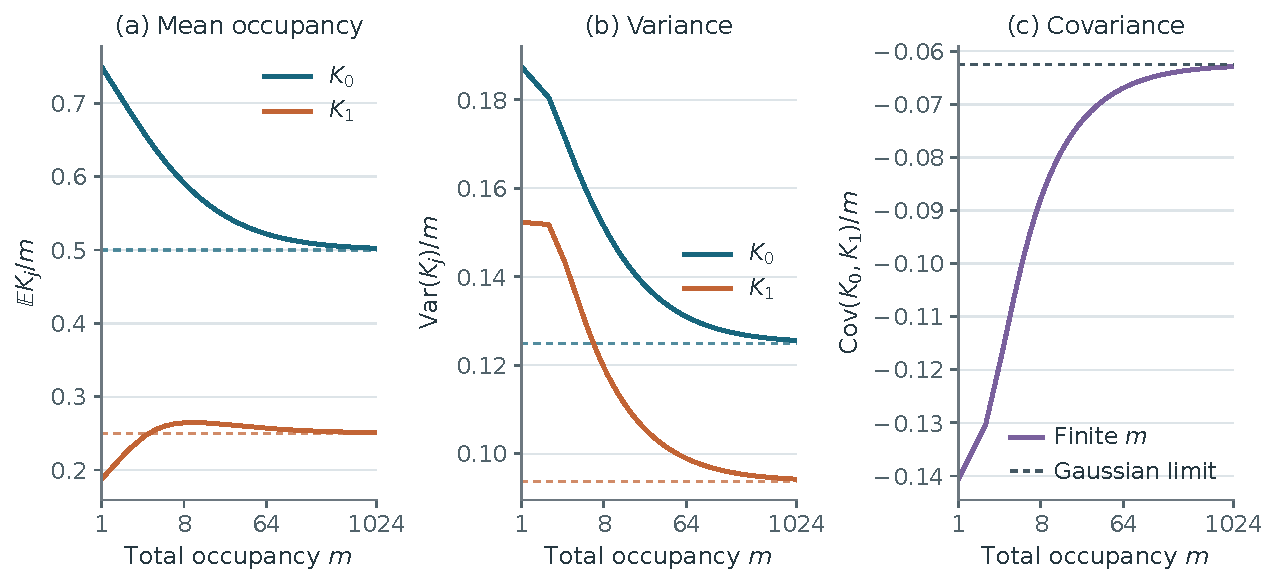
\includegraphics[width=\textwidth]{figures/occupancy_convergence.pdf}
\caption{The dyadic mean profile, variances, and covariance through
$m=1024$. Solid curves use the finite moment recurrence; dashed lines
show the proved limiting constants.}
\label{fig:bulk}
\end{figure}

\subsection{The global error constant}
For $q=1/2$, \cref{eq:l1-error} gives
\begin{equation}
C_{1/2}=\frac1{\sqrt\pi}\sum_{j\ge0}
 \sqrt{2^{-j-1}(1-2^{-j-1})}
\approx1.187645633962268.
\label{eq:dyadic-l1-constant}
\end{equation}
The omitted positive tail in this displayed numerical evaluation is at
most $8.56\times10^{-16}$; this does not include floating-point rounding.
The finite values of $\sqrt m\,\E\|K^{(m)}/m-c\|_1$ are
$1.2014456933$, $1.2084721023$, $1.2006282002$, and $1.1936305171$
for $m=16,64,256,1024$, respectively. Convergence need not be monotone.
Their omitted coordinate tails, after this scaling, are less than
$10^{-11}$.

To bound those omitted tails, let $R_{J+1}$ be the total remaining after
sites $0,\ldots,J$ in the exact residual-total chain. Then
\[
\sum_{j>J}\E|K_j-mc_j|\le\E R_{J+1}+mq^{J+1}.
\]
This deterministic inequality controls truncation without treating a small
spatial digit coefficient as a bound on an occupancy probability.

\subsection{Frontier checks and finite occupied counts}
The saddle is computed from the exact infinite-sum equation, not replaced
by $2m$. At $q=1/2$ and $m=1024$ it is
\[
t_m\approx2059.508071235173,\qquad n_m=10,\qquad
\theta_m\approx0.008084064817.
\]
The finite maximum distribution is computed by extracting the degree-$m$
coefficient from a finite head product and dividing by the full coefficient
in \cref{eq:partition}. The resulting errors against
\cref{eq:max-cdf} are shown in \cref{tab:frontier-errors}.

\begin{table}[htbp]
\centering
\caption{Maximum difference between the finite maximum-index CDF and its
moving-phase approximation on the tested integer range $s=-3,\ldots,5$.
These are measured errors on that range, not global error bounds.}
\label{tab:frontier-errors}
\begin{tabular}{@{}rr@{}}
\toprule
$m$ & Maximum absolute CDF difference \\
\midrule
16 & 0.012993410556 \\
64 & 0.004041664656 \\
256 & 0.001110769695 \\
1024 & 0.000285608694 \\
\bottomrule
\end{tabular}
\end{table}

At $m=1024$, the exact finite recurrences give
\[
\E H_m\approx9.508421724209,\qquad
\Var H_m\approx0.556160513709.
\]
The moving-phase predictions in \cref{eq:count-moments} are
$9.508071235173$ and $0.557174668735$, respectively. Numerically integrating
the limiting functions over phase gives $-1$ for the mean correction and
$0.557304959111037$ for the variance, agreeing with the exact expressions
in \cref{eq:phase-averages}.

\begin{figure}[htbp]
\centering
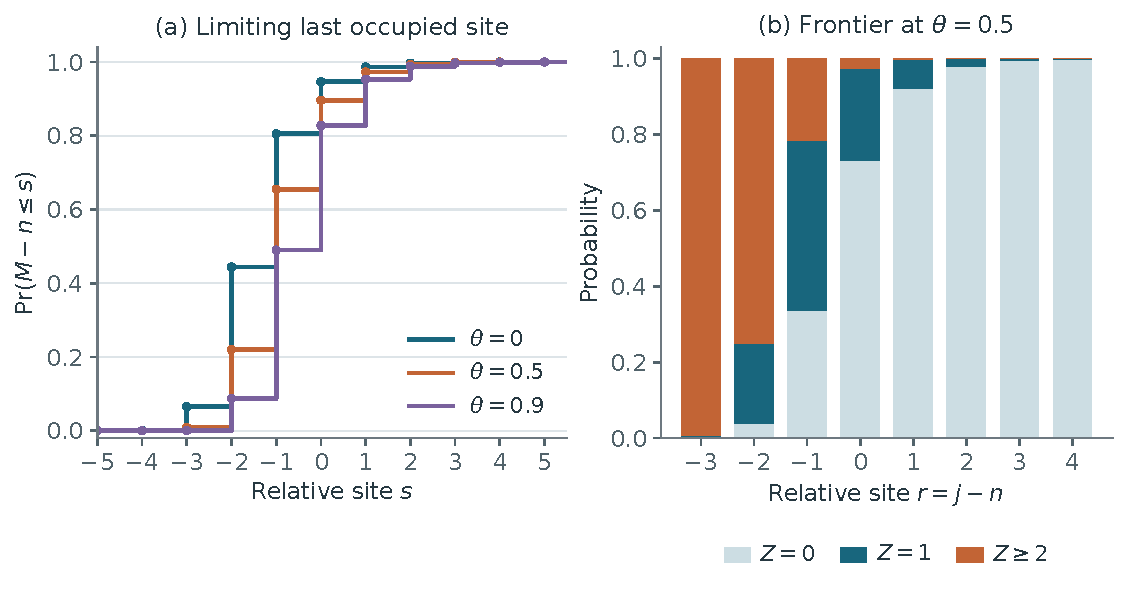
\includegraphics[width=0.98\textwidth]{figures/frontier_limits.pdf}
\caption{The discrete geometric frontier at $q=1/2$. Left: the limiting
maximum CDF for three phases, showing why the phase must be retained.
Right: the limiting occupancy probabilities near the frontier for phase
$\theta=1/2$. These panels display the explicit limiting laws, not sampled
finite configurations.}
\label{fig:frontier}
\end{figure}

\subsection{Numerical reliability and limitations}
The program's verification record reports maximum relative disagreement
$5.78\times10^{-15}$ between small exact moments and their floating
evaluations, maximum raw marginal normalization defect
$4.00\times10^{-15}$, and maximum absolute saddle-equation residual
$4.41\times10^{-13}$ for the selected levels. The omitted saddle tail is
bounded by $2.00\times10^{-15}$, and the omitted logarithmic maximum-CDF
tail by $1.98\times10^{-16}$. These analytic tail bounds do not enclose
all rounding or quadrature errors; the computation is not interval
arithmetic.

The tail bounds follow from elementary inequalities
\begin{equation}
\mu(a)\le\frac{a^2}{6},\qquad
0\le\log\frac{\sinh a}{a}\le\frac{a^2}{6}.
\label{eq:numeric-tail-bounds}
\end{equation}
For the first, compare positive power-series coefficients in
$a\cosh a-\sinh a\le(a^2/3)\sinh a$; the coefficient inequality
at degree $2k+1$ reduces to $3\le2k+1$ for $k\ge1$.
Divide by $2\sinh a$. The second follows by integrating
$\frac{\mathrm d}{\mathrm da}\log(\sinh a/a)=2\mu(a)/a\le a/3$.
Summing the resulting geometric tails gives the bounds used in the code.

\section{Further research questions and formalization plan}
\label{sec:questions}

The selected occupancy conjecture is proved in
\cref{thm:main-geometric}. The following questions concern stronger,
different, or more uniform statements. They are not assumptions in any
preceding proof.

\begin{question}[Effective local and global error bounds]
Can the uniform local limit theorem be made effective with explicit
constants in $q$ and $m$, and can the frontier total-variation error be
bounded by $C_q/m$ or $C_q(\log m)/m$? The numerical CDF errors in
\cref{tab:frontier-errors} suggest an inverse-$m$ scale on the tested
range, but do not establish a global rate. A useful first target is a
third- and fourth-cumulant Fourier estimate that remains uniform after
deleting a bounded-mean tail.
\end{question}

\begin{question}[An Edgeworth expansion for the bridge]
Determine the first nonzero correction to the finite Gaussian bridge
law, with the logarithmic saddle displacement and its phase retained.
Then determine which weighted sequence norms allow a corresponding
expansion. An expansion of the total normalizing coefficient alone is
insufficient: the marked coordinate transforms and the conditioning
likelihood must be expanded together.
\end{question}

\begin{question}[Quantitative independence of bulk and frontier]
Find an explicit distance between the joint law in
\cref{eq:joint-limit} and the product of its two limits. A particularly
concrete observable is the covariance between a fixed centered occupancy
and $H_m-\log_bm$. The theorem proves asymptotic independence in
distribution but does not give its first finite-$m$ interaction term.
\end{question}

\begin{question}[The dense-scale limit $q\uparrow1$]
The fixed-$q$ frontier variance has phase average
$(2\log2-1)/\log(1/q)$, which diverges as $q\uparrow1$.
What are the joint limits when $q=q_m\uparrow1$ with $m$?
One expects a transition from a bounded discrete frontier to an
approximately continuous occupied-count fluctuation. The regime of
validity of the retained-coordinate Fourier bound must be checked as
$c_0=1-q_m$ tends to zero.
\end{question}

\begin{question}[Nongeometric moving fronts]
For regularly varying weights, the number of sites with $t_mc_j$ of
order one grows with $m$, and the geometric lattice-phase description
changes. Determine the correct point-process or empirical-field limit,
its coupling to the $\ell^2$ bridge, and the fluctuations of the number
of occupied sites. The centering transition in \cref{thm:power} gives
one constraint that any such result must respect.
\end{question}

\begin{question}[Other symmetric digit laws]
Replace the uniform digits by symmetric compactly supported variables
with known endpoint behavior. The moment allocation formula in
\cref{eq:radial-derivative} survives, but the elementary hyperbolic
local factors are replaced by their even moment transforms. Which
endpoint hypotheses preserve amplitude limit shapes, Gaussian bridge
covariances, and entropy rates? Identify conditions that exclude extra
saddles or failure of a span-one local limit theorem.
\end{question}

\begin{question}[Other factorial residue classes]
For allocation weights involving $(dk+r)!$ in place of $(2k+1)!$,
with $d\ge2$, derive an analogue using Poisson variables conditioned
to a residue class. The present proof suggests covariance scaled by
$1/d$ and entropy rate $d\KL(p\|c)$ in suitable settings. Proving a
uniform Fourier estimate at all lattice peaks, especially with mixtures
of residue classes, is the necessary next step; no such general theorem
is claimed here.
\end{question}

\begin{question}[Exact sampling with a certified infinite tail]
The conditioning probability is asymptotic to $1/\sqrt{\pi m}$.
Can a sampler exploit the independent representation, the deterministic
geometric tail, and the explicit frontier to obtain exact samples with
near-linear or better expected work in the effective number of sites?
An approximate sampler should report a total-variation error for the
occupancy vector itself. A small omitted coefficient in the underlying
real random series is not such a certificate.
\end{question}

\begin{question}[Moderate deviations and sharp entropy asymptotics]
Between the $\sqrt m$ Gaussian scale and the speed-$m$ large deviation
principle, establish a moderate deviation principle in sequence spaces.
For fixed atypical profiles, derive the polynomial prefactor and the
boundary corrections to $\exp(-2m\KL(p\|c))$.
Infinite-entropy profiles and profiles with a growing number of occupied
coordinates will require separate uniformity arguments.
\end{question}

\begin{question}[The remaining zero-bias conjectures]
The source report also proposes spectral non-reappearance, a Bessel--Airy
zero transition, all-order phase-resolved Gaussianization of the transformed
real variable, and monotonicity of a standardized Stein discrepancy.
They concern different observables. Resolving the allocation conjecture
does not resolve those four statements. It would be useful to determine
which can use the joint bridge/frontier representation and which require
independent analytic input.
\end{question}

\subsection{A concrete formalization sequence}
The present proof separates into reusable layers. A Lean implementation
could proceed in the following order.
\begin{enumerate}
\item \textbf{Finite algebra.} Formalize the local hyperbolic series,
the factorial identity, the finite coefficient normalization, and the
finite conditional probability formula. These are suitable for exact
checks before any asymptotic library is needed.
\item \textbf{Countable probability.} Construct independent $B_a$ laws;
prove almost-sure finiteness of $S(t)$, positivity of the conditioning
event, and passage from finite coefficients to \cref{eq:conditioning}.
\item \textbf{Scalar analysis.} Establish the moment formulas, variance
bounds, the unique saddle, and the global characteristic-function bound.
\item \textbf{Fourier inversion.} Prove the lattice local limit theorem
using an $L^1$ dominated-convergence lemma for rescaled characteristic
functions. This is the key reusable asymptotic component.
\item \textbf{Sequence-space convergence.} Combine finite block
conditioning with the uniform omitted-coordinate bound, first in
$\ell^2$, then in $\ell^1$, and formalize the Gaussian necessity
argument for square-root summability.
\item \textbf{Geometric and entropy layers.} Add the moving-tail
total-variation theorem, defect-field moment bounds, and the separate
large deviation proof through finite partitions and explicit compact
sets.
\end{enumerate}
No code in this package is represented as a Lean proof. The numerical
script and its rational assertions verify finite examples, while the
article specifies the mathematical obligations for a future formalization.

\appendix
\section{Repository provenance and reproduction}
\label{app:provenance}

The source report is linked in \cite{repo-report}. It lies in the
\texttt{Fabius\_Zero\_Bias\_Frontier\_Report} directory under the
representations drafts in \texttt{Analysis/FabiusFunction/docs}.
At the inspected repository commit
\texttt{a21208b3ff14a07a4c8318dbf916d543acbef043}, its Git blob identifier is
\texttt{3e406ee42205a5ea223863c2bfbd4c0a8cece08a}.
The exact labels used to identify the problem are
\texttt{eq:q-occupancy}, \texttt{eq:occupancy-partition},
\texttt{conj:occupancy-shape}, \texttt{eq:occupancy-LLN}, and
\texttt{eq:occupancy-CLT}. The accompanying source README explicitly
distinguishes the report's paper-level claims from the formal Lean corpus.

The package contains this self-contained LaTeX source and its compiled
PDF, the numerical program, dependency requirements, numerical notes,
the CSV/JSON records, and the two figures in PDF and PNG form.
No third-party article or repository source is redistributed.

To regenerate the computations, run from the extracted package:
\begin{verbatim}
python -m pip install -r requirements.txt
python verify_occupancy.py
\end{verbatim}
The recorded run used Python 3.12.14, NumPy 2.3.5, SciPy 1.17.0, and
Matplotlib 3.10.8. The program records its actual runtime versions in
\texttt{data/verification\_summary.json}. The provided requirements
specify compatible minimum versions; reproducing the recorded version
set is preferable when comparing the last printed digits. Exact rational
identities are independent of floating-point versions.

To rebuild the article, keep the supplied \texttt{figures/} directory
beside the source and run:
\begin{verbatim}
pdflatex -interaction=nonstopmode -halt-on-error occupancy_article.tex
pdflatex -interaction=nonstopmode -halt-on-error occupancy_article.tex
pdflatex -interaction=nonstopmode -halt-on-error occupancy_article.tex
\end{verbatim}
The bibliography is embedded in the source. It requires no BibTeX run,
network access, or repository-specific notation file.

\begin{thebibliography}{9}
\raggedright
\interlinepenalty=10000

\bibitem{repo-report}
V. Reshetnikov, \emph{ProveIt} repository, Fabius--Rvachev research corpus.
\emph{Zero-Bias Towers and Spectral Peeling in the Fabius--Rvachev System},
source manuscript and accompanying README; in particular
\texttt{conj:occupancy-shape}.
Repository snapshot \texttt{a21208b3ff14a07a4c8318dbf916d543acbef043},
inspected 5 October 2026 (UTC).
\href{\sourceURL}{Pinned source manuscript};
\href{\repoURL}{repository home}.

\bibitem{goldstein-reinert}
L. Goldstein and G. Reinert,
Stein's method and the zero bias transformation with application to simple
random sampling, \emph{Annals of Applied Probability} \textbf{7} (1997),
935--952.
\href{https://doi.org/10.1214/aoap/1043862419}{doi:10.1214/aoap/1043862419}.
\href{https://arxiv.org/abs/math/0510619}{arXiv:math/0510619}
(electronic deposit, 2005).

\bibitem{arratia-tavare}
R. Arratia and S. Tavar\'e,
Independent process approximations for random combinatorial structures,
\emph{Advances in Mathematics} \textbf{104} (1994), 90--154.
\href{https://doi.org/10.1006/aima.1994.1022}{doi:10.1006/aima.1994.1022}.
\href{https://arxiv.org/abs/1308.3279}{arXiv:1308.3279}
(electronic deposit, 2013).

\bibitem{gnedin-hansen-pitman}
A. Gnedin, B. Hansen, and J. Pitman,
Notes on the occupancy problem with infinitely many boxes: general
asymptotics and power laws,
\emph{Probability Surveys} \textbf{4} (2007), 146--171.
\href{https://doi.org/10.1214/07-PS092}{doi:10.1214/07-PS092}.
\href{https://arxiv.org/abs/math/0701718}{arXiv:math/0701718}.

\bibitem{flajolet-gourdon-dumas}
P. Flajolet, X. Gourdon, and P. Dumas,
Mellin transforms and asymptotics: harmonic sums,
\emph{Theoretical Computer Science} \textbf{144} (1995), 3--58.
\href{https://doi.org/10.1016/0304-3975(95)00002-E}
{doi:10.1016/0304-3975(95)00002-E}.

\bibitem{arias}
J. Arias de Reyna,
An infinitely differentiable function with compact support: definition
and properties,
\href{https://arxiv.org/abs/1702.05442}{arXiv:1702.05442} (2017),
English version of work originally published in Spanish in 1982.

\end{thebibliography}
\end{document}
